\documentclass[11pt]{article}
\usepackage[a4paper, margin=2.54cm]{geometry}
\usepackage[utf8]{inputenc}
\usepackage[spanish, mexico]{babel}
\usepackage[spanish]{layout}
\usepackage[article]{ragged2e}
\usepackage{textcomp}
\usepackage{caption}
\usepackage{subcaption}
\usepackage{graphicx}
\usepackage{multirow}
\usepackage{amsmath}
\usepackage{amsfonts}
\usepackage{yhmath}
\usepackage{mathtools}
\usepackage{blkarray, bigstrut}
\def\Big#1{\makebox(0,0){\huge#1}}

% ============================================================================
% ============================================================================
% ============================================================================

\title{
  TRABAJO PRÁCTICO FINAL\\
  \large Probabilidad y Estadística
}
\author{
  Farizano, Juan Ignacio \\
  \and
  Mellino, Natalia
}
\date{}

% ============================================================================
% ============================================================================
% ============================================================================

\begin{document}

\maketitle
\newpage

\tableofcontents
\newpage

% ============================================================================
% ============================================================================
% ============================================================================

\section{Ejercicio 1}

\subsection*{Apartado a)}

Para realizar la simulación utilizamos la siguiente función en R, donde recibe 
como parámetro la probabilidad $ p $ de que salga cara al tirar la moneda. Como
la moneda está equilibrada, en este caso la función tomará $ p = 0.5 $.

\begin{verbatim}
  simularCienTiradas <- function(P) {
    Sim <- sample(c("Cara", "Cruz"), 100, T, c(P, 1 - P))
    length(which(Sim == "Cara"))
  }
\end{verbatim}

Evaluando una vez esta función con parámetro $ p = 0.5 $ obtenemos:

\begin{verbatim}
  > simularCienTiradas(0.5)
  [1] 54
\end{verbatim}

En esta simulación el número de caras resultó ser 54.

% ============================================================================

\subsection*{Apartado b)}

Este apartado se puede resolver de dos formas distintas: una utilizando
la simulación y otra usando la teoría vista en clase. Para este apartado
interpretamos a $ X $ como $ X_{100} $.

\subsubsection*{Utilizando la simulación:}

Para hallar la $ P(X = 1) $ y la $ E(X) $ utilizamos el siguiente código, 
donde los argumentos recibidos $ N $ y $ P $ representan la cantidad de veces
que se simularán las cien tiradas (siendo N arbitrariamente grande) y P
es análoga al apartado a). En la función la variable \texttt{Acumulador}
es la suma de la cantidad de veces que salió cara en todas las simulaciones
y la variable \texttt{Uno} representa la cantidad de veces que una simulación
dió un numero de caras igual a uno.

\begin{verbatim}
  simularCienPorN <- function(N, P) {
    Acumulador <- 0
    Uno <- 0
    for (i in 1:N) {
      Sim <- simularCienTiradas(P)
      Acumulador <- Acumulador + Sim
      if (Sim == 1) {
        Uno <- Uno + 1
      }
    }
    c(Uno / N, Acumulador / N)
  }
\end{verbatim}

Cuando ejecutamos esta función, obtenemos los siguientes resultados:

\begin{verbatim}
  > simularCienPorN(1000000, 0.5)
  [1]  0.00000 49.98931
\end{verbatim}

Al intentar estimar los valores pedidos con la simulación, se obtuvo que
la $ P(X) = 1 $ es aproximadamente 0 (esto lo veremos al calcular el valor
de forma teórica, lo que sucede es que la probabilidad es tan chica que en
ninguna simulación sucede). Por otro lado, estimamos el valor de la esperanza
que se acerca a 50, que como veremos luego, éste es el valor exacto.

\subsubsection*{Utilizando la teoría:}

Para calcular $ P(X = 1) $ definimos una nueva variable aleatoria
$ Y $: número de caras obtenidas de un total de 100. Entonces, hallar
$ P(X = 1) $ es igual a hallar $ P(Y = 1) $, donde $ Y $ tiene una \textbf{Distribución
Binomial} de parámetros $ n = 100, \; p = 0.5 $, es decir, $ Y \sim B(100, 0.5) $.

\begin{align*}
  P(Y = 1) &= \binom{100}{1} \cdot 0.5^1 \cdot (1 - 0.5)^{100 - 1} \\
           &= 100 \cdot 0.5 \cdot 0.5^{99} \\
           &= 7.888609052 \cdot 10^{-29}
\end{align*}

Por lo tanto, $ P(X = 1) =  7.888609052 \cdot 10^{-29}$, que como podemos ver
es muy pequeña, y eso explica que no hayamos obtenido una buena estimación con
nuestra simulación.

Para hallar la esperanza de $ X $, hacemos:

\begin{equation*}
    E(X) = E(Y) = n \cdot p = 100 \cdot 0.5 = 50
\end{equation*}

Y así podemos afirmar que nuestra simulación pudo obtener una buena estimación
para $ E(X) $.

% ============================================================================

\subsection*{Apartado c)}

En este apartado, también se realizó de forma teórica y utilizando la simulación.

\subsubsection*{Utilizando la simulación}

Utilizamos el siguiente código:

\begin{verbatim}
  tresCaras <- function(N, P) {
    Acumulador <- 0
    for (i in 1:N) {
      Veces <- 0
      Tiradas <- 0
      while(Veces < 3) {
        Sim <- sample(c("Cara", "Cruz"), 1, T, c(P, 1 - P))
        if (Sim[1] == "Cara") {
          Veces <- Veces + 1
        }
        Tiradas <- Tiradas + 1
      }
      Acumulador <- Acumulador + Tiradas
    }
    Acumulador / N
  }
\end{verbatim}

y obtenemos el siguiente resultado:

\begin{verbatim}
  > buscarTres(1000000, 0.5)
  [1] 6.004526
\end{verbatim}

Entonces, se obtuvo que el número de veces a realizar el experimento hasta
obtener 3 caras es aproximadamente 6.

\subsubsection*{Utilizando la teoría}

Definimos una nueva variable aleatoria, $ Z $: número de veces que se realizó el
experimento hasta que salió cara por tercera vez. Esta variable aleatoria posee
una \textbf{distribución de Pascal} de parámetros $ r = 3 $ y $ p = 0.5 $. Lo que queremos
hallar nosotros entonces, es el número promedio de veces que se realizó el 
experimento hasta que salió cara por tercera vez, es decir, queremos hallar
$ E(Z) $, que viene dado por:

\begin{equation*}
  E(Z) = \frac{r}{p} = \frac{3}{0.5} = 6
\end{equation*}

Por lo tanto, el número promedio de veces que se deberá realizar el experimento hasta
que salga cara por tercera vez es 6.

% ============================================================================

\subsection*{Apartado d):}

El código dado en los apartados a) y b) ya permite que la moneda sea sesgada,
a continuación, realizamos la simulación parados valores diferentes de $ p $:
$ p = 0.01 $, $ p = 0.3 $ y $ p = 0.85 $

\begin{verbatim}
  simularCienPorN(1000000, 0.01)
  [1] 0.369727 1.000360

  > simularCienPorN(1000000, 0.3)
  [1]  0.00000 29.99997

  > simularCienPorN(1000000, 0.85)
  [1]  0.0000 84.9958
\end{verbatim}

De estas simulaciones, obtuvimos los siguientes resultados:

\begin{table}[h!]
  \begin{center}
    \begin{tabular}{| c | r | r |}
      \hline
      $ p $ & $ P(X = 1) $ & $ E(X) $ \\ \hline
      $ 0.01 $ & $ 0.3697 $ & $ 1.0003 $ \\ \hline
      $ 0.03 $ & $ 0.0000 $ & $ 29.9999 $ \\ \hline
      $ 0.85 $ & $ 0.0000 $ & $ 84.9958 $ \\ \hline 
    \end{tabular}
  \end{center}
\end{table}

% ============================================================================
% ============================================================================
% ============================================================================

\section{Ejercicio 2}

\subsection*{Apartado a)}
Para simular el proceso $ D_n $ utilizamos la siguiente función escrita en R

\begin{verbatim}
  trayectoriaD <- function(N, P) {
    Sim <- sample(c(1, 0), N, T, c(P, 1 - P))
    D <- vector()
    for (i in 1:N) {
      D[i] <- 2 * Sim[i] - 1
    }
    D
  }
\end{verbatim}

Para simular 10 pasos de una trayectoria de $ D_n $ (suponiendo que la moneda
está equilibrada) realizamos lo siguiente
\begin{verbatim}
  > trayectoriaD(10, 0.5)
  [1]  1  1 -1 -1  1  1  1  1 -1 -1
\end{verbatim}

% ============================================================================

\subsection*{Apartado b)}
Para simular el proceso $ S_n $ utilizamos la siguiente función escrita en R

\begin{verbatim}
  trayectoriaS <- function(N, P) {
    D <- trayectoriaD(N, P)
    S <- c(D[1])
    for (i in 2:N) {
      S[i] <- S[i - 1] + D[i]
    }
    S
  }
\end{verbatim}

Simulamos una trayectoria utilizando los mismos parámetros que en el apartado
a) y graficamos

\begin{figure}[h!]
  \begin{center}
    \begin{subfigure}[b]{\linewidth}
      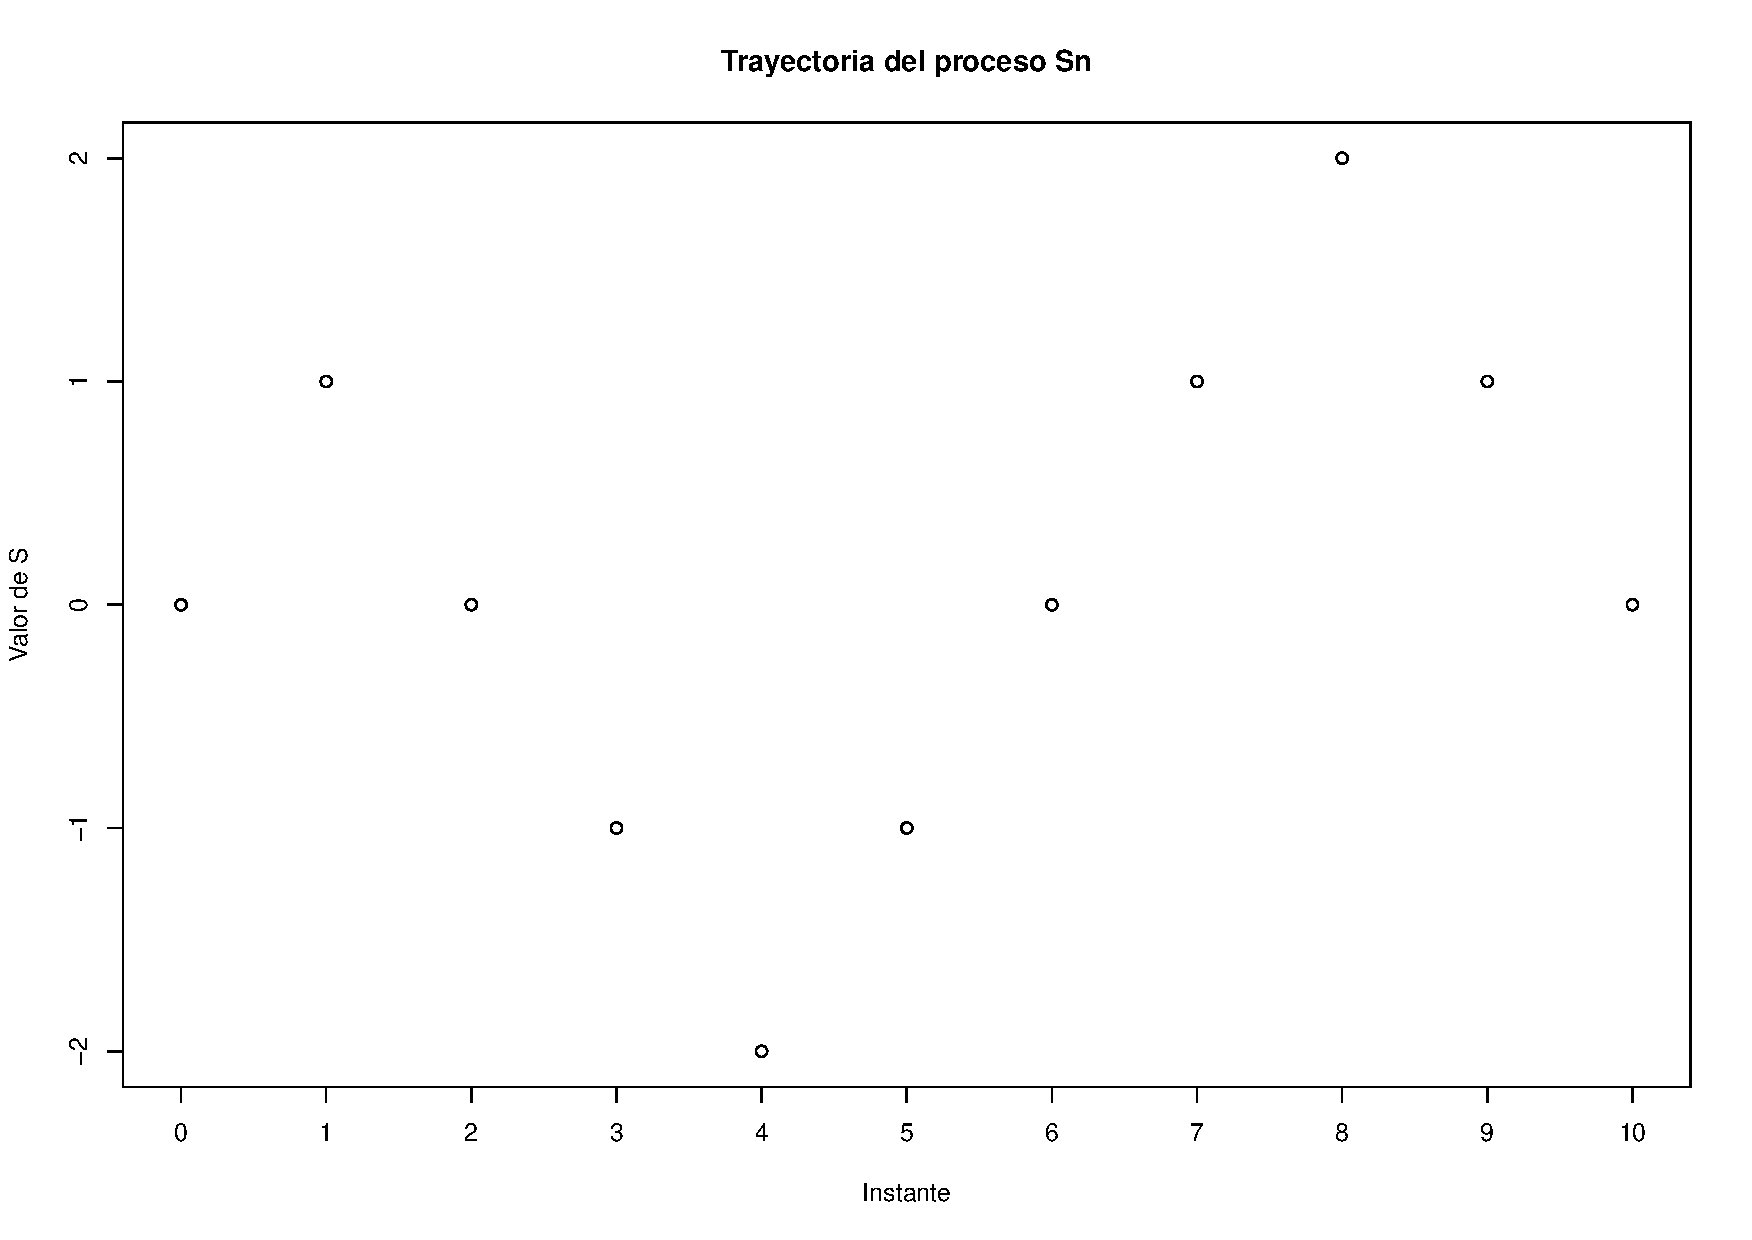
\includegraphics[width=\linewidth]{trayectoriaS.pdf}
    \end{subfigure}
  \end{center}
\end{figure}

% ============================================================================
% ============================================================================
% ============================================================================

\section{Ejercicio 3}

\subsection*{Apartado a)}

Para simular la trayectoria del jugador utilizamos el siguiente código en R:

\begin{verbatim}
  gamblersRuinTrayectoria <- function(P, K, S) {
    Pasos = 0
    Resultado = K
    Trayectoria = c(K)
    
    while (Resultado != 0 & Resultado != S) {
      Resultado = Resultado + sample(c(1, -1), 1, T, c(P, 1 - P))[1]
      Trayectoria = c(Trayectoria, Resultado)
      Pasos = Pasos + 1
    }
  }
\end{verbatim}

% =====================================================0.9=======================

\subsection*{Apartado b)}

Utilizando el código escrito en a) con los valores $P = 0.6, \; K = 35, \; S = 100$ obtuvimos el
siguiente gráfico

\begin{figure}[h!]
  \begin{center}
    \begin{subfigure}[b]{\linewidth}
      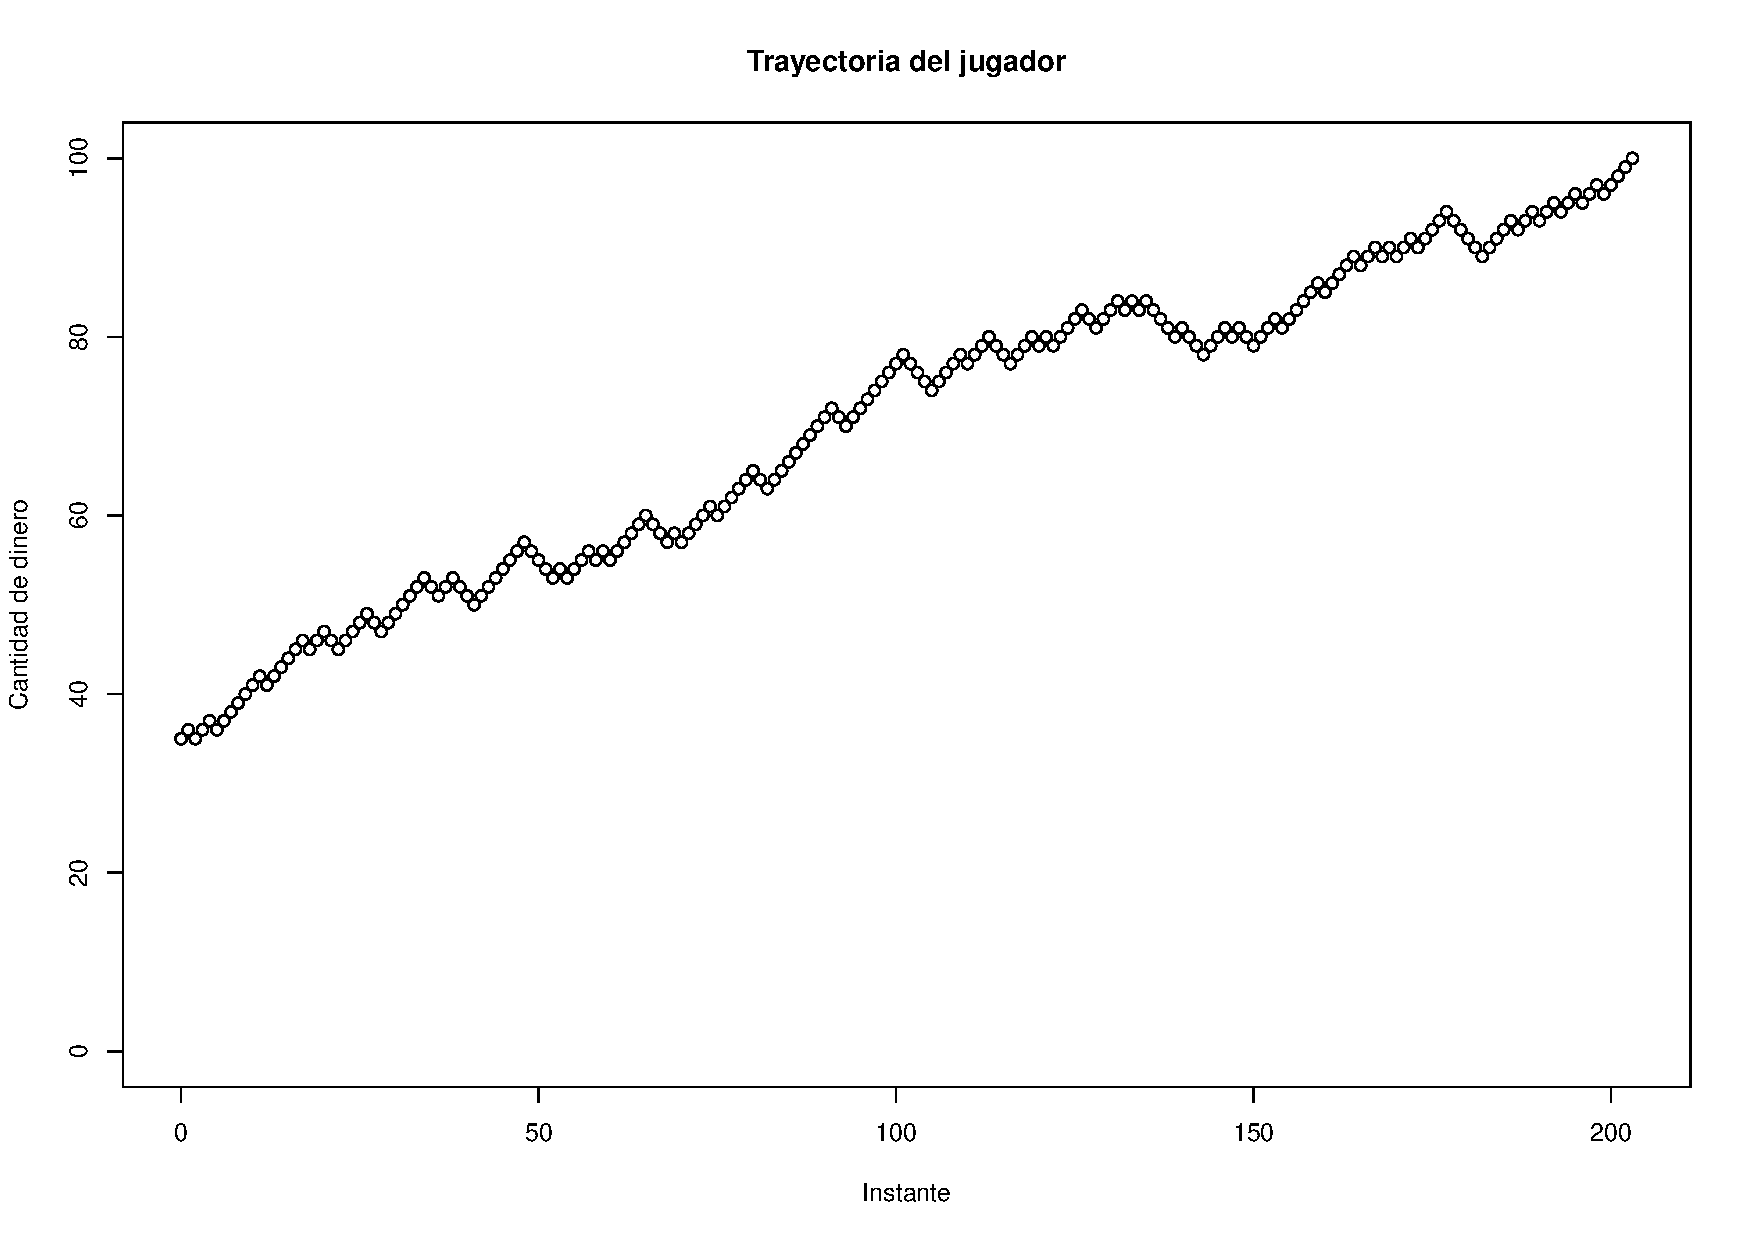
\includegraphics[width=\linewidth]{trayectoriaGamblers.pdf}
    \end{subfigure}
  \end{center}
\end{figure}

% ============================================================================

\subsection*{Apartado c):}

Resolvemos este apartado por simulación y luego comprobamos los resultados teóricamente.
Tomamos los valores: $ k = 3, \; S = 5,\; p = 0.65 $.

\subsubsection*{Simulación}

\begin{verbatim}
  calcularProbRuinaIter <- function(P, K, S, Simulaciones) {
    Arruinado <- 0
    for (i in 1:Simulaciones) {
      Resultado <- K
      Pasos <- 0

      while (Resultado != 0 & Resultado != S) {
        Resultado <- Resultado + sample(c(1, -1), 1, T, c(P, 1 - P))[1]
        Pasos <- Pasos + 1
      }
      if (Resultado == 0) {
        Arruinado <- Arruinado + 1
      }
    }
    Arruinado / Simulaciones
  }
\end{verbatim}

Y obtenemos como resultado:

\begin{verbatim}
  > calcularProbRuinaIter(0.65, 3, 5, 100000)
  [1] 0.11564
\end{verbatim}

\subsubsection*{Teórico}

Podemos modelar el problema como una Cadena de Markov estados: E = \{0, 1, 2, 3, 4, 5\},
donde la matriz de transición es:

\begin{equation*}
  P = 
  \begin{blockarray}{cccccccc}
     & & 0 & 1 & 2 & 3 & 4 & 5 \\
    \begin{block}{cc(cccccc)}
      0 & & 1    & 0    & 0    & 0    & 0    & 0 \\
      1 & & 0.35 & 0    & 0.65 & 0    & 0    & 0 \\
      2 & & 0    & 0.35 & 0    & 0.65 & 0    & 0 \\
      3 & & 0    & 0    & 0.35 & 0    & 0.65 & 0 \\
      4 & & 0    & 0    & 0    & 0.35 & 0    & 0.65 \\
      5 & & 0    & 0    & 0    & 0    & 0    & 1 \\
    \end{block}
  \end{blockarray}
\end{equation*}

Queremos estimar la probabilidad de ruina del jugador, esto es hallar la $ F(k = 3, 0) $. 
Vimos en teoría que:

\begin{equation*}
  G(i, \; j) = F(i, \;, k) \; \forall k \in C_j
\end{equation*}

Sabemos que $ G = SB $, donde $ S = (I - Q)^{-1} $. Entonces procedemos a 
calcular las matrices correspondientes:

\begin{equation*}
  Q = 
  \begin{blockarray}{cccccc}
     & & 1 & 2 & 3 & 4 \\
    \begin{block}{cc(cccc)}
      1 & & 0    & 0.65 & 0    & 0    \\
      2 & & 0.35 & 0    & 0.65 & 0    \\
      3 & & 0    & 0.35 & 0    & 0.65 \\
      4 & & 0    & 0    & 0.35 & 0    \\
    \end{block}
  \end{blockarray}
\end{equation*}

\begin{equation*}
  B = 
  \begin{blockarray}{cccc}
     & & 0 & 5 \\
    \begin{block}{cc(cc)}
      1 & & 0.35 & 0   \\
      2 & & 0    & 0   \\
      3 & & 0    & 0   \\
      4 & & 0    & 0.65 \\
    \end{block}
  \end{blockarray}
\end{equation*}

\begin{equation*}
  S = 
  \begin{blockarray}{cccccc}
     & & 1 & 2 & 3 & 4 \\
    \begin{block}{cc(cccc)}
      1 & & 1.4759 & 1.3598 & 1.1441 & 0.7437 \\
      2 & & 0.7322 & 2.0920 & 1.7602 & 1.1441 \\
      3 & & 0.3317 & 0.9478 & 2.0920 & 1.3598 \\
      4 & & 0.1161 & 0.3317 & 0.7322 & 1.4759 \\
    \end{block}
  \end{blockarray}
\end{equation*}

\begin{equation*}
  G = 
  \begin{blockarray}{cccc}
     & & 0 & 5 \\
    \begin{block}{cc(cc)}
      1 & & 0.5165 & 0.4834 \\
      2 & & 0.2562 & 0.7437 \\
      3 & & 0.1161 & 0.8838 \\
      4 & & 0.0406 & 0.9593 \\
    \end{block}
  \end{blockarray}
\end{equation*}

Entonces, la probabilidad de ruina del jugador arracando con $ k = 3 $ es $ G(3, 0) \simeq 0.1161 $ (los resultados de la 
matriz $S$ y $G$ están redondeados a 4 cifras decimales). Observemos además que con la simulación
se obtuvo una buena aproximación a la probabilidad deseada.

% ============================================================================
% ============================================================================
% ============================================================================

\section{Ejercicio 4}

\subsection*{Apartado a)}

Realizamos la simulación utilizando el siguiente código en R, siendo el 
argumento N la cantidad de veces que se realizará la simulación:

\begin{verbatim}
  ratonLaboratorio <- function(N) {
    Total = 0

    for (i in 1:N) {
      Tiempo = 0
      Resultado = "Seguir"

      while (Resultado == "Seguir") {
        Direccion = sample(c("Izquierda", "Derecha"), 1, T, c(0.5, 0.5))[1]
        if (Direccion == "Izquierda") {
          Resultado = sample(c("Seguir", "Salir"), 1, T, c(2/3, 1/3))[1]
          if (Resultado == "Seguir") {
            Tiempo = Tiempo + 5
          } else {
            Tiempo = Tiempo + 2
            Resultado = "Salir"
          }
        } else {
          Tiempo = Tiempo + 3
        }

      }
      Total = Total + Tiempo
    }
  
    Total / N
}
\end{verbatim}

Al realizar la simulación un millón de veces, obtenemos el siguiente resultado:

\begin{verbatim}
  > ratonLaboratorio(1000000)
  [1] 20.98719
\end{verbatim}

% ============================================================================

\subsection*{Apartado b)}

Definimos las variables aleatorias: \\
\begin{center}
  X: tiempo (en minutos) que tarda el ratón en salir del laberinto.
\end{center}

\[
  Y = \begin{cases}
        1 & \text{si el ratón elige la puerta izquierda y va a la salida} \\
        2 & \text{si el ratón elige la puerta izquierda y vuelve al inicio} \\
        3 & \text{si el ratón elige la puerta derecha}
      \end{cases}
\]

Entonces, si queremos obtener el resultado del apartado a) en forma analítica simplemente recurrimos
a la fórmula de esperanza condicional:

\begin{align*}
  E(X) &= E(X \vert Y = 1)P(Y = 1) + E(X \vert Y = 2)P(Y = 2) + E(X \vert Y = 3)P(Y = 3) \\
       &= 2 \cdot \frac{1}{2} \cdot \frac{1}{3} + 
          (5 + E(X)) \cdot \frac{1}{2} \cdot \frac{2}{3} +
          (3 + E(X)) \cdot \frac{1}{2} \\
      &= \frac{1}{3} + \frac{5}{3} + \frac{E(X)}{3} + \frac{3}{2} + \frac{E(X)}{2} \\
      &= \frac{7}{2} + \frac{5}{6} \cdot E(X) \Rightarrow \frac{E(X)}{6} = \frac{7}{2} \Rightarrow E(X) = 21
\end{align*}

% ============================================================================
% ============================================================================
% ============================================================================

\section{Ejercicio 5}

\subsection*{Apartado a)}

Sea P la matriz de transición de la cadena

\begin{equation*}
  P = 
  \begin{blockarray}{ccccc}
     & \text{S} & \text{VIH} & \text{SIDA} & \text{M} \\
    \begin{block}{c(cccc)}
      \text{S}    & 0.999 & 0.001 & 0     & 0 \\
      \text{VIH}  & 0     & 0.994 & 0.006 & 0 \\
      \text{SIDA} & 0     & 0     & 0.918 & 0.082 \\
      \text{M}    & 0     & 0     & 0     & 1 \\
    \end{block}
  \end{blockarray}
\end{equation*}

Llamamos $E$ al conjunto de estados, luego $E =$ \{S, VIH, SIDA, M\}

A partir del grafo hallamos el conjunto cerrado al cual pertenece cada uno de
los estados.
\begin{itemize}
  \item $C_S$ = \{S, VIH, SIDA, M\} = $E$
  \item $C_{VIH}$ = \{VIH, SIDA, M\}
  \item $C_{SIDA}$ = \{SIDA, M\}
  \item $C_M =$ \{M\}
\end{itemize}

$C_S$, $C_{\text{VIH}}$ y $C_{\text{SIDA}}$ son conjuntos cerrados no irreducibles finitos,
$C_M$ es irreducible finito.
La CM no es irreducible y por lo tanto no es periódica, aperiódica, recurrente, transitoria ni ergódica.
Ningún estado es periódico.
S, VIH y SIDA son estados transitorios, M es un estado absorbente.

% ============================================================================

\subsection*{Apartado b)}

Viendo la matriz de transición podemos deducir lo siguiente:

\begin{align*}
&F(\text{VIH}, S) = F(\text{SIDA}, S) = F(\text{SIDA}, \text{VIH}) = F(M, S) = F(M, \text{VIH}) = F(M, \text{SIDA}) = 0 \\
&F(M, M) = 1
\end{align*}
entonces la matriz $ F $ nos queda completada parcialmente de la siguiente manera:

\begin{equation*}
  F = 
  \begin{blockarray}{ccccc}
     & \text{S} & \text{VIH} & \text{SIDA} & \text{M} \\
    \begin{block}{c(cccc)}
      \text{S}    & - & - & - & - \\
      \text{VIH}  & 0 & - & - & - \\
      \text{SIDA} & 0 & 0 & - & - \\
      \text{M}    & 0 & 0 & 0 & 1 \\
    \end{block}
  \end{blockarray}
\end{equation*}

Ahora, procedemos a hallar la matriz $ G = SB $:

\begin{equation*}
  Q = 
  \begin{blockarray}{cccc}
     & \text{S} & \text{VIH} & \text{SIDA} \\
    \begin{block}{c(ccc)}
      \text{S}    & 0.999 & 0.01  & 0 \\
      \text{VIH}  & 0     & 0.994 & 0.06 \\
      \text{SIDA} & 0     & 0     &  0.918   \\
    \end{block}
  \end{blockarray}
\end{equation*}

\begin{equation*}
  B = 
  \begin{blockarray}{cc}
     & C_M \\
    \begin{block}{c(c)}
      \text{S}    & 0 \\
      \text{VIH}  & 0 \\
      \text{SIDA} & 0.082   \\
    \end{block}
  \end{blockarray}
\end{equation*}

$ S = (I - Q)^{-1} $ 

\begin{equation*}
  S = 
  \begin{blockarray}{cccc}
     & \text{S} & \text{VIH} & \text{SIDA} \\
    \begin{block}{c(ccc)}
      \text{S}    & 1000 & 166.\overline{6} & 12.1951 \\
      \text{VIH}  & 0    & 166.\overline{6} & 12.1951 \\
      \text{SIDA} & 0    & 0                & 12.1951 \\
    \end{block}
  \end{blockarray}
\end{equation*}

Luego la matriz $ G = SB $ viene dada por: 

\begin{equation*}
  G = 
  \begin{blockarray}{cc}
     & C_M \\
    \begin{block}{c(c)}
      \text{S}    & 1 \\
      \text{VIH}  & 1 \\
      \text{SIDA} & 1  \\
    \end{block}
  \end{blockarray}
\end{equation*}

Luego, a partir de la matriz $G$ podemos deducir que:

$ F(S, M) = F(S, \text{VIH}) = F(S, \text{SIDA}) = 1 $

y podemos seguir completando la matriz $F$.

\begin{equation*}
  F = 
  \begin{blockarray}{ccccc}
     & \text{S} & \text{VIH} & \text{SIDA} & \text{M} \\
    \begin{block}{c(cccc)}
      \text{S}    & - & - & - & 1 \\
      \text{VIH}  & 0 & - & - & 1 \\
      \text{SIDA} & 0 & 0 & - & 1 \\
      \text{M}    & 0 & 0 & 0 & 1 \\
    \end{block}
  \end{blockarray}
\end{equation*}

Ahora, recordemos que la matriz $S$ es igual a la matriz $R$ suprimiendo las 
filas y columnas de estados recurrentes. 

\begin{equation*}
  R = 
  \begin{blockarray}{ccccc}
     & \text{S} & \text{VIH} & \text{SIDA} & \text{M}\\
    \begin{block}{c(cccc)}
      \text{S}    & 1000 & 166.\overline{6} & 12.1951 & -\\
      \text{VIH}  & 0    & 166.\overline{6} & 12.1951 & -\\
      \text{SIDA} & 0    & 0                & 12.1951 & -\\
      \text{M}    & -    & -                & -       & - \\
    \end{block}
  \end{blockarray}
\end{equation*}

Entonces como sabemos que $F(j, j) = 1 - \frac{1}{R(j, j)}$ y $F(i, j) = \frac{R(i, j)}{R(j, j)}$.
Ahora podemos completar lo que resta de la matriz:

\begin{itemize}
  \item $ F(S, S) = 0.999$
  \item $ F(S, \text{VIH}) = F(S, \text{SIDA}) = F(\text{VIH}, \text{SIDA}) = 1 $
  \item $ F(\text{SIDA}, \text{SIDA}) = 0.9179$
\end{itemize}
  
Y la matriz $F$ nos queda:

\begin{equation*}
  F = 
  \begin{blockarray}{ccccc}
     & \text{S} & \text{VIH} & \text{SIDA} & \text{M} \\
    \begin{block}{c(cccc)}
      \text{S}    & 0.999 & 1      & 1      & 1 \\
      \text{VIH}  & 0     & 0.9939 & 1      & 1 \\
      \text{SIDA} & 0     & 0      & 0.9179 & 1 \\
      \text{M}    & 0     & 0      & 0      & 1 \\
    \end{block}
  \end{blockarray}
\end{equation*}

Los datos que nos provee la matriz $F$ se pueden interpretar como la probabilidad
de pasar de un estado $e$ a un estado $e'$ en un tiempo en años finito.

% ============================================================================

\subsection*{Apartado c)}

Basta hacer el siguiente calculo:

$ A = S1 $ donde $1$ es el vector columna cuyas entradas son el número $1$

\begin{equation*}
  A = 
  \begin{blockarray}{cc}
     & \text{M} \\
    \begin{block}{c(c)}
      \text{S}    & 1178.8617 \\
      \text{VIH}  & 178.8617 \\
      \text{SIDA} & 12.1951 \\
    \end{block}
  \end{blockarray}
\end{equation*}

Esto lo podemos interpretar de la siguiente manera: \\
La entrada $A(e, 1)$ con $e \in$ \{S, VIH, SIDA\} representa el tiempo promedio en años
que le tomará pasar de el estado $e$ a estar muerto (pasar al estado M).

% ============================================================================

\newpage
\subsection*{Apartado d)}

Para hallar la distribución invariante planteamos el siguiente sistema
de ecuaciones:

\begin{itemize}
  \item $\pi P = \pi$
  \item $\displaystyle\sum_{i \in E} \pi(i) = 1$
\end{itemize}

\[
\begin{cases}
  0.999a = a \\
  0.001a + 0.994b=b \\
  0.006b+0.918c=c \\
  0.082c+d = d \\
  a+b+c+d=1 \\
\end{cases}
\]

Utlizando un solucionador de ecuaciones online, obtenemos el vector $\pi$

\begin{equation*}
  \pi = 
  \begin{blockarray}{cccc}
     \text{S} & \text{VIH} & \text{SIDA} & \text{M} \\
    \begin{block}{(cccc)}
      0 & 0 & 0 & 1 \\
    \end{block}
  \end{blockarray}
\end{equation*}

Por lo tanto, para esta cadena sí existe una distribución invariante.

% ============================================================================

\subsection*{Apartado e)}

La matriz P ya se encuentra descompuesta en su forma canónica:

\begin{equation*}
  P = 
  \begin{blockarray}{ccccc}
    & \text{S} & \text{VIH} & \text{SIDA} & \text{M} \\
   \begin{block}{c(ccc|c)}
     \text{S}    & & & & \\
     \text{VIH}  & & \Big{Q} & & \Big{B} \\
     \text{SIDA} & & & & \\
     \cline{2-5}
     \text{M}    & & 0 & & I \\
   \end{block}
  \end{blockarray}
  \;\; =
  \begin{blockarray}{ccccc}
     & \text{S} & \text{VIH} & \text{SIDA} & \text{M} \\
    \begin{block}{c(ccc|c)}
      \text{S}    & 0.999 & 0.001 & 0     & 0 \\
      \text{VIH}  & 0     & 0.994 & 0.006 & 0 \\
      \text{SIDA} & 0     & 0     & 0.918 & 0.082 \\
      \cline{2-5}
      \text{M}    & 0     & 0     & 0     & 1 \\
    \end{block}
  \end{blockarray}
\end{equation*}

Con la ayuda del siguiente lema podremos calcular la distribución límite: \\

\textbf{Lema:} Sea A una matriz cuadrada tal que $ A^n \rightarrow 0 $ cuando
$ n \rightarrow \infty $, entonces:

\begin{equation*}
  \sum_{n = 0}^{\infty} A^n = (I - A)^{-1}
\end{equation*}

Y ayudándonos de la multiplicación por bloques de matrices, tenemos lo siguiente:

\begin{equation*}
  P^n = 
  \begin{blockarray}{cc}
   \begin{block}{(c|c)}
    Q^n & (I + Q + \dots + Q^{n-1})B \\
    \cline{1-2}
    0 & I \\
   \end{block}
  \end{blockarray}
\end{equation*}

Entonces como $ Q^n \rightarrow 0 $ cuando $ n \rightarrow 0 $ podemos usar el lema auxiliar
para hallar $ \displaystyle\lim_{n \rightarrow \infty} P^n $:

\begin{align*}
  \displaystyle\lim_{n \rightarrow \infty} P^n &=
  \begin{blockarray}{cc}
    \begin{block}{(c|c)}
     Q^n & (I + Q + \dots + Q^{n-1})B \\
     \cline{1-2}
     0 & I \\
    \end{block}
   \end{blockarray} \\
  & =
  \begin{blockarray}{cc}
    \begin{block}{(c|c)}
     \displaystyle\lim_{n \rightarrow \infty} Q^n & \displaystyle\lim_{n \rightarrow \infty} (I + Q + \dots + Q^{n-1})B \\
     \cline{1-2}
     0 & I \\
    \end{block}
   \end{blockarray} \\
  & = 
  \begin{blockarray}{cc}
    \begin{block}{(c|c)}
     0 & (I - Q)^{-1}B \\
     \cline{1-2}
     0 & I \\
    \end{block}
  \end{blockarray} \\
\end{align*}

Realizando los calculos con nuestra matriz mediante uso de un software obtenemos:

\begin{equation*}
  \displaystyle\lim_{n \rightarrow \infty} P^n =
  \begin{blockarray}{ccccc}
    & \text{S} & \text{VIH} & \text{SIDA} & \text{M} \\
   \begin{block}{c(cccc)}
     \text{S}    & 0 & 0 & 0 & 1 \\
     \text{VIH}  & 0 & 0 & 0 & 1 \\
     \text{SIDA} & 0 & 0 & 0 & 1 \\
     \text{M}    & 0 & 0 & 0 & 1 \\
   \end{block}
 \end{blockarray}
\end{equation*}

Por lo tanto la distribución límite viene dada por el siguiente vector fila, que
coincide con la distribución invariante obtenida en el apartado d).

\begin{equation*}
  \pi = 
  \begin{blockarray}{cccc}
     \text{S} & \text{VIH} & \text{SIDA} & \text{M} \\
    \begin{block}{(cccc)}
      0 & 0 & 0 & 1 \\
    \end{block}
  \end{blockarray}
\end{equation*}

\section{Ejercicio 6}

\subsection*{Apartado a)}

Podemos transformar el grafo dado en el enunciado en una Cadena de Markov,
si asumimos que cualquier página A que no tiene hipervínculos tiene igual 
probabilidad de ir a todas las páginas (A incluida). Entonces, en el grafo
de la figura, basta con agregar aristas desde $g$ a todas las páginas
distribuyendo uniformemente la probabilidad. 
La matriz de transición P de la cadena nos queda de la siguiente forma:

\begin{equation*}
  P = 
  \begin{blockarray}{cccccccc}
     & \text{a} & \text{b} & \text{c} & \text{d} & \text{e} & \text{f} & \text{g} \\
    \begin{block}{c(ccccccc)}
      \text{a} & 0           & 0           & 0           & 0           & \frac{1}{2} & \frac{1}{2} & 0 \\
      \text{b} & \frac{1}{3} & 0           & \frac{1}{3} & 0           & 0           & \frac{1}{3} & 0 \\
      \text{c} & 0           & 0           & 0           & \frac{1}{2} & 0           & \frac{1}{2} & 0 \\
      \text{d} & 0           & 0           & 0           & 0           & 0           & 1           & 0 \\
      \text{e} & \frac{1}{4} & 0           & 0           & \frac{1}{4} & 0           & \frac{1}{4} & \frac{1}{4} \\
      \text{f} & \frac{1}{2} & \frac{1}{2} & 0           & 0           & 0           & 0           & 0 \\
      \text{g} & \frac{1}{7} & \frac{1}{7} & \frac{1}{7} & \frac{1}{7} & \frac{1}{7} & \frac{1}{7} & \frac{1}{7} \\
    \end{block}
  \end{blockarray}
\end{equation*}

% ============================================================================

\newpage
\subsection*{Apartado b)}

Para realizar la simulación, utilizamos la siguiente función en R:
\begin{verbatim}
  simPageRank <- function() {
    States <- as.character(1:7)
    P <<- matrix(c(0, 0, 0, 0, 1/2, 1/2, 0, 
                  1/3, 0, 1/3, 0, 0, 1/3, 0,
                  0, 0, 0, 1/2, 0, 1/2, 0,
                  0, 0, 0, 0, 0, 1, 0,
                  1/4, 0, 0, 1/4, 0, 1/4, 1/4,
                  1/2, 1/2, 0, 0, 0, 0, 0,
                  1/7, 1/7, 1/7, 1/7, 1/7, 1/7, 1/7), nrow = 7, ncol = 7, byrow = T,
                dimnames = list(States, States))
    MC <<- new("markovchain", states = States, transitionMatrix = P, name="PageRank")
    pi <- c(1/7, 1/7, 1/7, 1/7, 1/7, 1/7, 1/7)
    Sim <<- rmarkovchain(MC, n = 100, t0 = sample(States, 1, T, pi)[1])
  }
\end{verbatim}

Simulamos 100 pasos del proceso y obtuvimos el siguiente recorrido:

\begin{figure}[h!]
  \begin{center}
    \begin{subfigure}[b]{\linewidth}
      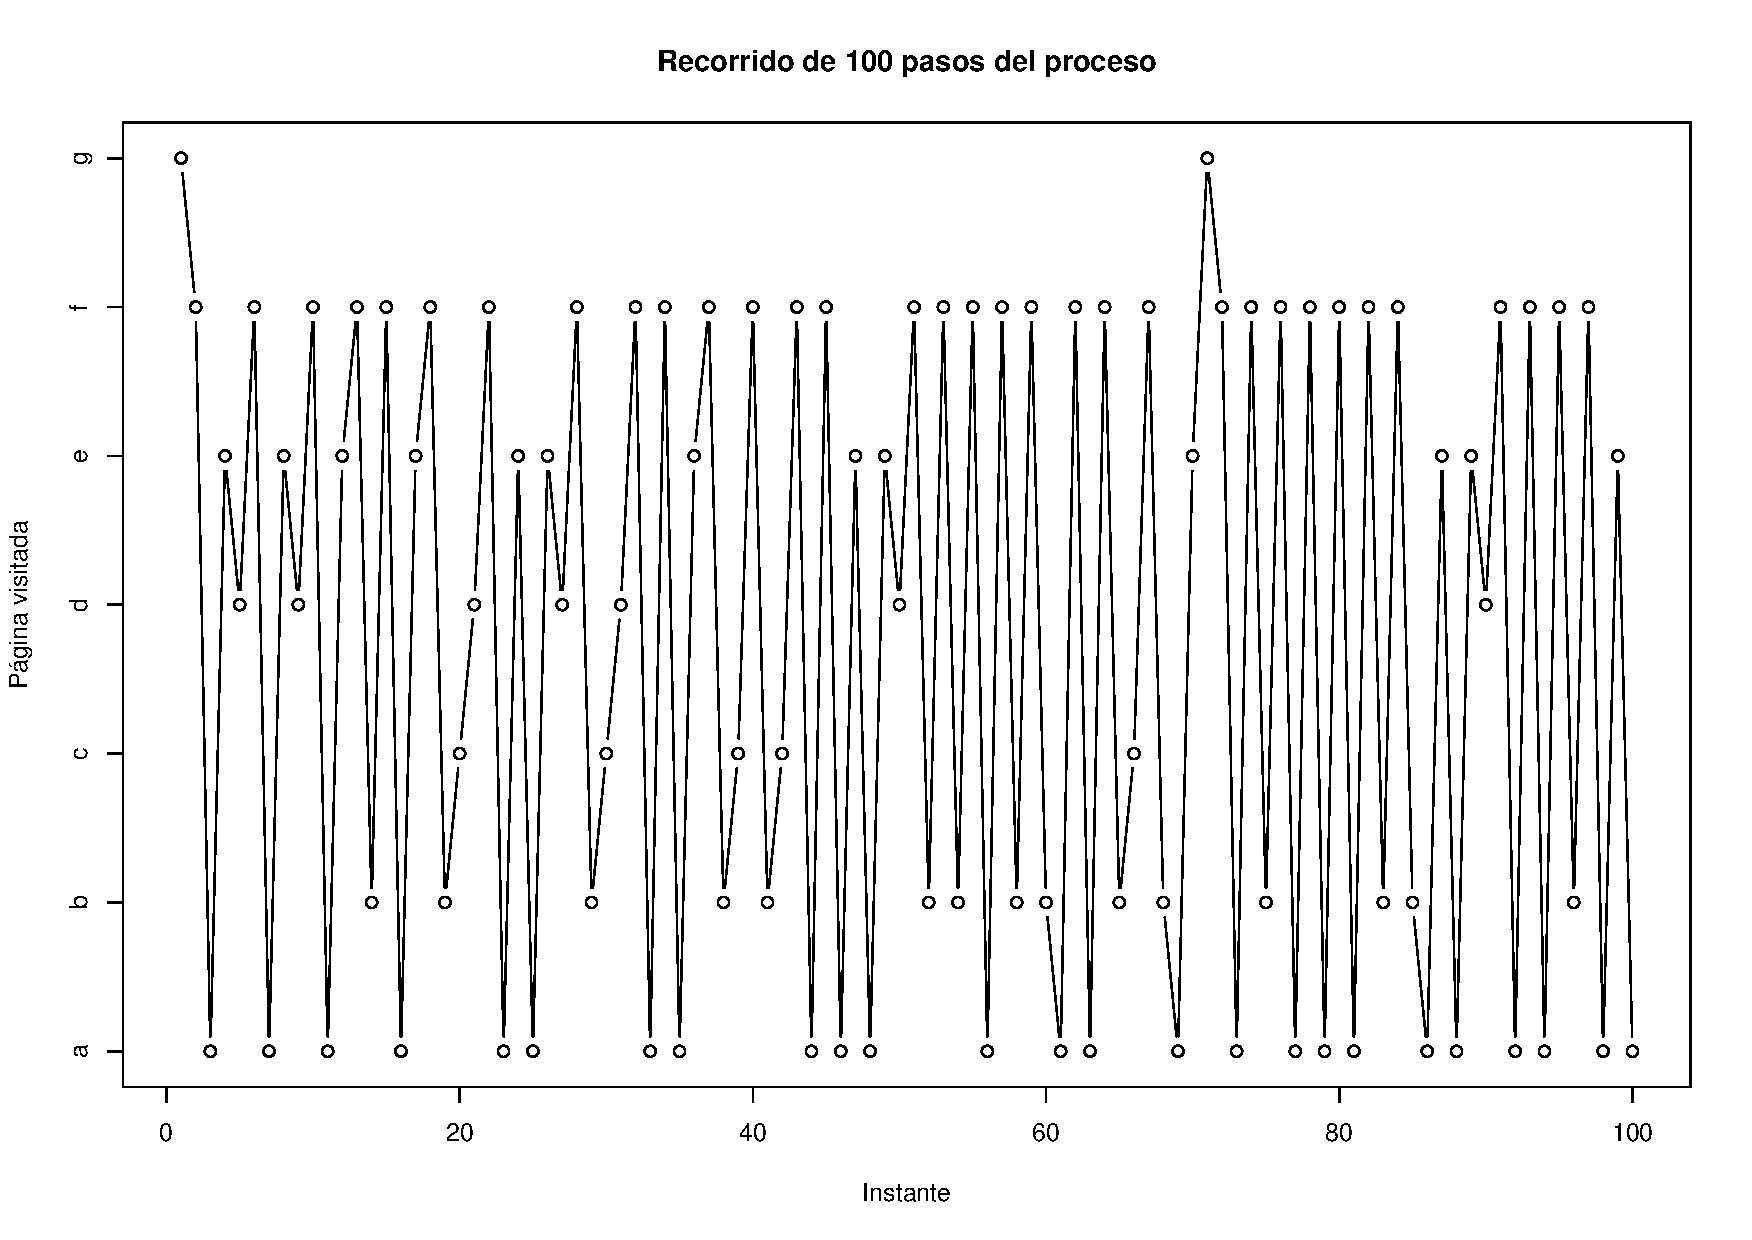
\includegraphics[width=\linewidth]{recorridoPageRank.pdf}
    \end{subfigure}
  \end{center}
\end{figure}


% ============================================================================

\subsection*{Apartado c)}

El rango de cada página es la probabilidad a largo plazo de permanecer en ella,
entonces, para encontrarlo necesitamos hallar su distribución límite. Como la matriz
es irreducible y aperiódica podemos hallar la distrubución encontrando
$\pi$ tal que cumpla con el siguiente sistema de ecuaciones:

\begin{itemize}
  \item $\pi P = \pi$
  \item $\displaystyle\sum_{i \in E} \pi(i) = 1$
\end{itemize}

Usando la función steadyStates de la librería de cadenas de markov obtenemos:

\begin{equation*}
  \pi = 
  \begin{blockarray}{ccccccc}
    \text{a} & \text{b} & \text{c} & \text{d} & \text{e} & \text{f} & \text{g} \\
    \begin{block}{(ccccccc)}
      0.2440318 & 0.1591512 & 0.05835544 & 0.066313 & 0.127321 & 0.3076923 & 0.03713528 \\
    \end{block}
  \end{blockarray}
\end{equation*}

% ============================================================================
% ============================================================================
% ============================================================================

\section{Ejercicio 7}

\subsection*{Apartado a)}

Podemos definir $N_t$ como un proceso de Poisson de parámetro $\lambda = 10$ que
cuenta la cantidad de mensajes que llegaron en el intervalo [0, t], con $t_0 = 10:00hs, \;
t_1 = 11:00hs$, etc. Dicho proceso cumple las siguientes hipótesis:

\begin{enumerate}
  \item El número de mensajes recibidos durante intervalos de tiempo
        no sobrepuestos son variables aleatorias independientes.
  \item Si tenemos otra variable $ M_t $ que representa el número de 
        mensajes recibidos en un intervalo $[t_1, t_1 + t]$ para cualquier
        $ t_1 > 0 $, entonces ambas variables tienen la misma distribución de
        probabilidades. Es decir, la distribución depende sólo de la longitud
        del intervalo.
  \item Si definimos $p_n(t) = P(N_t = n)$. Tenemos que si $\Delta_t$
        es suficientemente pequeño entonces $p_1(\Delta_t) \simeq \lambda \Delta_t$. 
        Esto quiere decir, que la probabilidad de recibir exactamente un mensaje en
        ese intervalo es directamente proporcional a la longitud del intervalo.
  \item $\displaystyle\sum_{k = 2}^{\infty} p_k(\Delta_t) \simeq 0 $ esto 
        implica que $ p_k(\Delta_t) \rightarrow 0 $, $k \geq 2$.
        Esto significa que la probabilidad de recibir dos o más
        mensajes en un intervalo suficientemente pequeño es despreciable.
  \item $ N_0 = 0 $, o equivalentemente, $ p_0(0) = 1 $.
\end{enumerate}

Queremos hallar $ P(N_2 = 18, N_7 = 70) $, observemos que si entran 18 mensajes en
el intervalo $[0, 2]$ y 70 en el $[0, 7]$, entonces entran $70 - 18 = 52$ mensajes en
el intervalo $(2, 7]$, entonces tenemos ahora que los intervalos $[0, 2] $ y $ (2, 7] $
son disjuntos y entonces se tiene que:

\begin{align*}
  P(N_2 = 18, N_7 = 70) &= P(N_2 = 18, N_7 - N_2 = 52) \\
                        &= P(N_2 = 18) \cdot P(N_7 - N_2 = 52) \\
                        &= P(N_2 = 18) \cdot P(N_5 = 52) \\
                        &= \frac{e^{-2(10)} \cdot (2 \cdot 10)^{18}}{18!} \cdot \frac{e^{-5(10)} \cdot (5 \cdot 10)^{52}}{52!} \\
                        &= 0.0045
\end{align*}

Por lo tanto la probabilidad de que reciba 18 mensajes el mediodía y 70 a la tarde es de 0.0045.

% ============================================================================

\newpage

\subsection*{Apartado b)}

Mediante el siguiente código en R realizamos una simulación del proceso:

\begin{verbatim}
  ej7 <- function(t) {
    i <- 1
    X <- c(rexp(1, 10))
    S <- c(X[1])
    
    while (S[i] <= t) {
      i <- i + 1
      X[i] <- rexp(1, 10)
      S[i] <- X[i] + S[i - 1]
      
    }
  }
\end{verbatim}

En el gráfico de abajo podemos ver la trayectoria de la simulación realizada
con un tiempo $t = 48$:

\begin{figure}[h!]
  \begin{center}
    \begin{subfigure}[b]{\linewidth}
      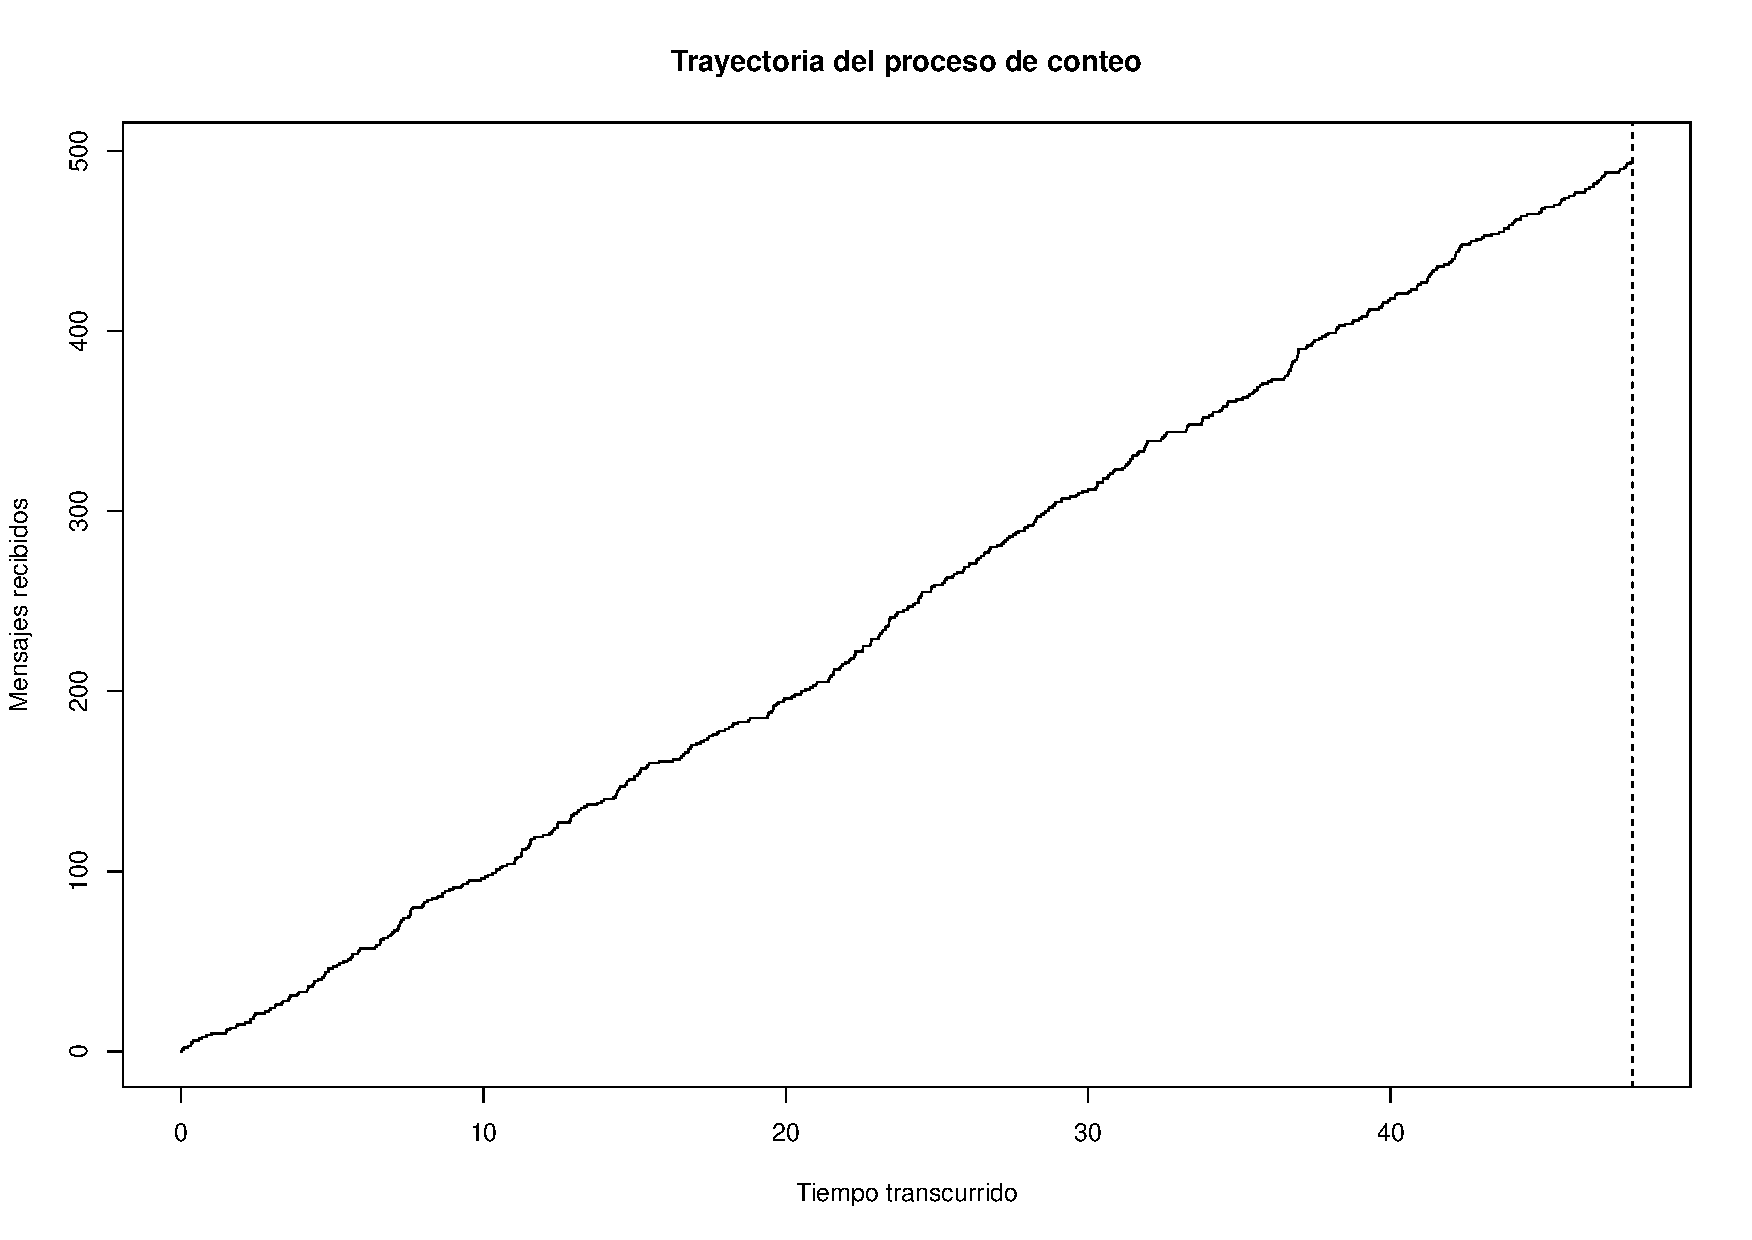
\includegraphics[width=\linewidth]{trayectoriaMensajes.pdf}
    \end{subfigure}
  \end{center}
\end{figure}

En el siguiente histograma representamos los tiempos entre llegadas en el
intervalo [0, 48], comparándolo con la función teórica de densidad del tiempo (en horas)
interarribos.

\begin{figure}[h!]
  \begin{center}
    \begin{subfigure}[b]{\linewidth}
      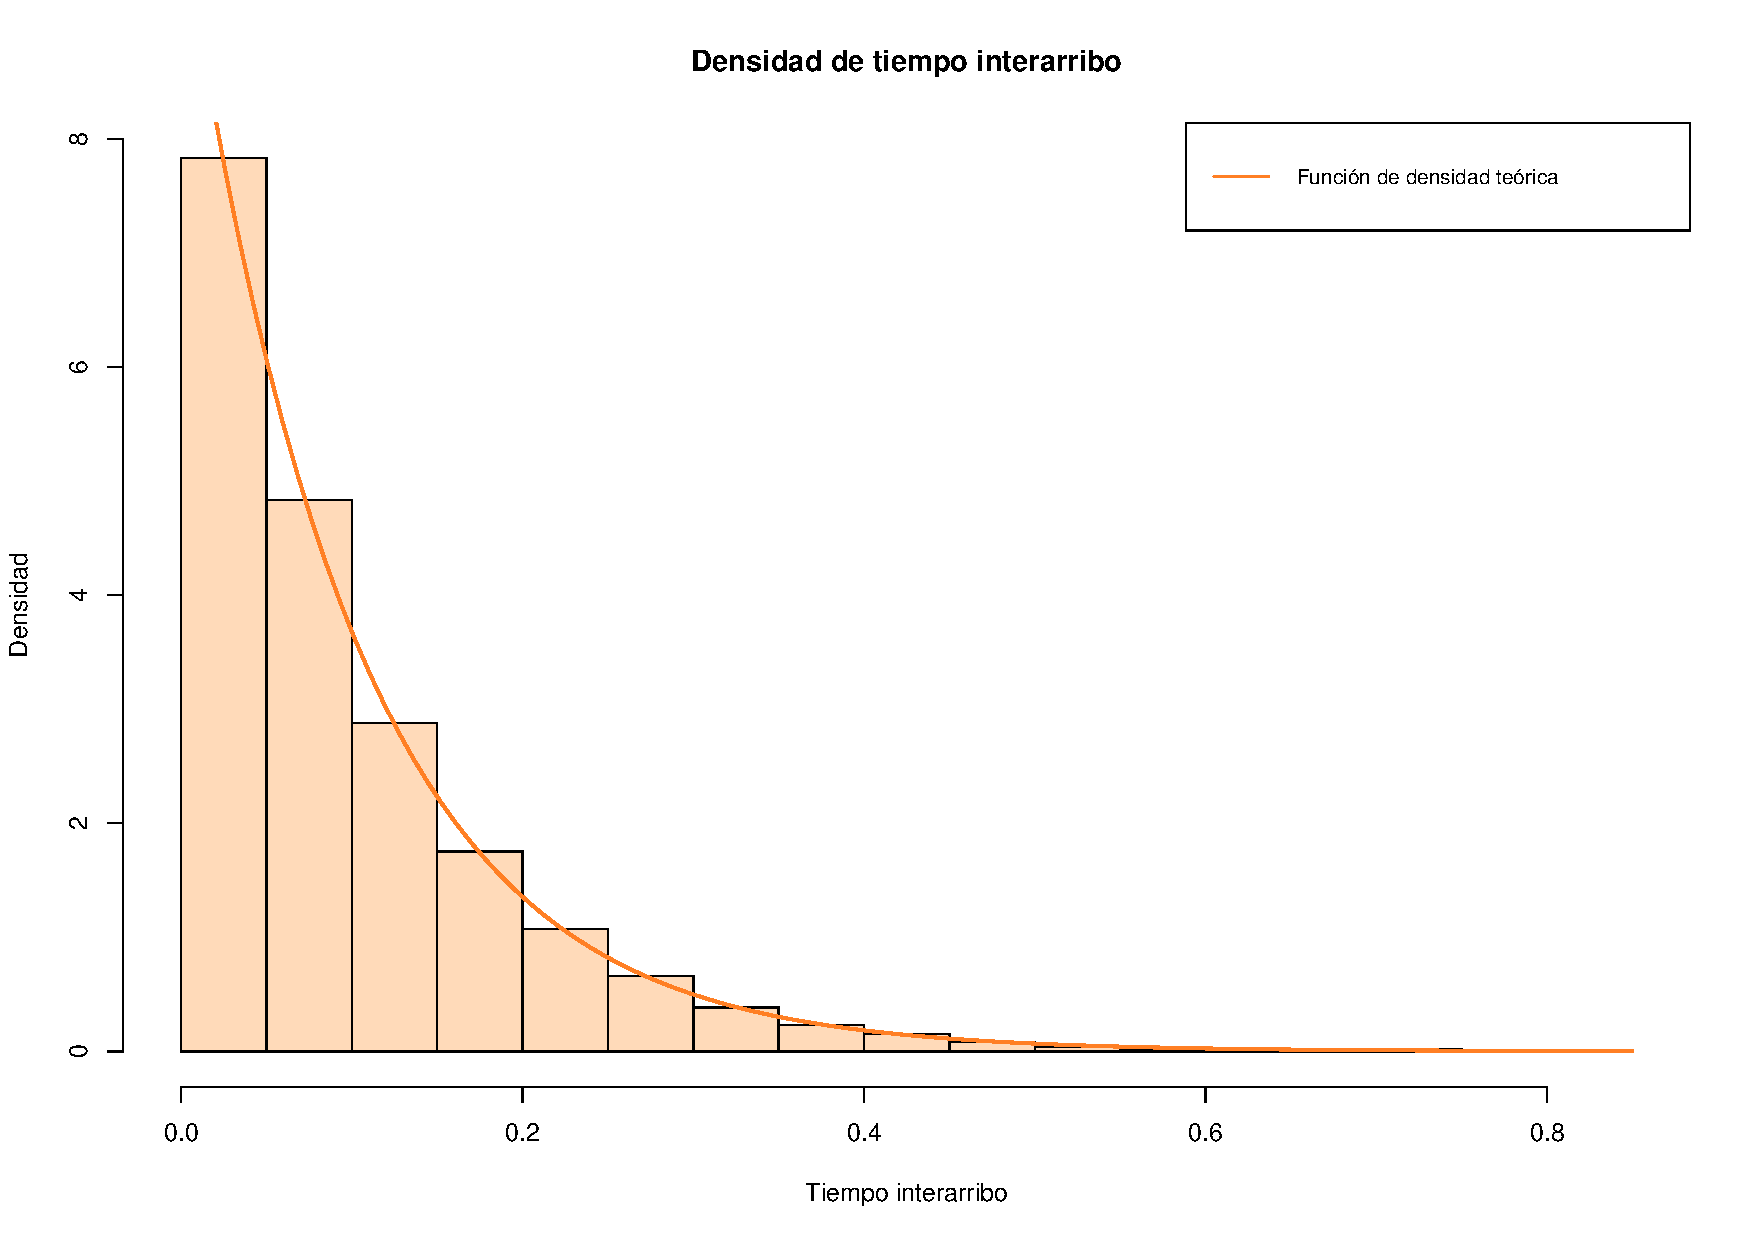
\includegraphics[width=\linewidth]{densidadTiempoInterarribo.pdf}
    \end{subfigure}
  \end{center}
\end{figure}


% ============================================================================
% ============================================================================
% ============================================================================

\newpage

\section{Ejercicio 8}

\subsection*{Apartado a)}

Sea P la matriz de transición.

\begin{equation*}
  P = 
  \begin{blockarray}{ccccccc}
    & & 80 & 135 & 139 & 445 & \text{No attack} \\
    \begin{block}{cc(ccccc)}
      80        & & 0            & 0            & 0            & 0            & 1 \\
      135       & & 0            & \frac{8}{13} & \frac{3}{13} & \frac{1}{13} & \frac{1}{13} \\
      139       & & \frac{1}{16} & \frac{3}{16} & \frac{3}{8}  & \frac{1}{4}  & \frac{1}{8} \\
      445       & & 0            & \frac{1}{11} & \frac{4}{11} & \frac{5}{11} & \frac{1}{11} \\
      \text{No} & & 0            & \frac{1}{8}  & \frac{1}{2}  & \frac{1}{8}  & \frac{1}{4} \\
    \end{block}
  \end{blockarray}
\end{equation*}

y sea el vector de distribución inicial $\pi_0 = (0, 0, 0, 0, 1)$

Para obtener la probabilidad de cada estado después de dos semanas debemos calcular
la matriz de transición en 2 pasos $\pi_0 \cdot P^2$ y obtenemos:

\begin{equation*}
  \begin{blockarray}{ccccc}
    80 & 135 & 139 & 445 & \text{No attack} \\
    \begin{block}{(ccccc)}
      0.03125 & 0.2132867 & 0.3868007 & 0.2226836 & 0.145979 \\
    \end{block}
  \end{blockarray}
\end{equation*}

Por lo tanto, el puerto con más probabilidad de ser atacado después de dos semanas
es el puerto 139, y el menos probable es el puerto 90.

% ============================================================================

\subsection*{Apartado b)}

Podemos verificar en R que la matriz es aperiódica, irreducible y finita, 
resultando ser ergódica:

\begin{verbatim}
  > period(MC)
  [1] 1

  > is.irreducible(MC)
  [1] TRUE  
\end{verbatim}

Por lo tanto, la distribución invariante es única, resulta ser la distribución
límite y viene dada por la solución al sistema de ecuaciones:

\begin{itemize}
  \item $\pi P = \pi$
  \item $\displaystyle\sum_{i \in E} \pi(i) = 1$
\end{itemize}

Sea $ \pi = (a, b, c, d, e) $, planteamos el sistema de ecuaciones
\[
\begin{cases}
  \frac{1}{16}c = a \\
  \frac{8}{13}b + \frac{3}{16}c + \frac{1}{11}d + \frac{1}{8}e = b \\
  \frac{3}{13}b + \frac{3}{8}c + \frac{4}{11}d + \frac{1}{2}e = c \\
  \frac{1}{13}b + \frac{1}{4}c + \frac{5}{11}d + \frac{1}{8}e = d \\
  a + \frac{1}{13}b + \frac{1}{8}c + \frac{1}{11}d + \frac{1}{4}e = e \\
  a + b + c + d + e = 1 \\
\end{cases}
\]

Resolviendo el sistema obtenemos que

\begin{equation*}
  \pi = 
  \begin{blockarray}{ccccc}
    80 & 135 & 139 & 445 & \text{No attack} \\
    \begin{block}{(ccccc)}
      0.02146667 & 0.2669333 & 0.3434667 & 0.2273333 & 0.1408 \\
    \end{block}
  \end{blockarray}
\end{equation*}

\end{document}